%package list
\documentclass{article}
\usepackage[utf8]{inputenc}
\usepackage[top=3cm, bottom=3cm, outer=3cm, inner=3cm]{geometry}
\usepackage{multicol}
\usepackage{graphicx}
\usepackage{url}

%\usepackage{cite}
\usepackage{hyperref}
\usepackage{array}

%\usepackage{multicol}
\newcolumntype{x}[1]{>{\centering\arraybackslash\hspace{0pt}}p{#1}}
\usepackage{natbib}
\usepackage{pdfpages}
\usepackage{multirow}
\usepackage[normalem]{ulem}
\useunder{\uline}{\ul}{}
\usepackage{svg}
\usepackage{xcolor}
\usepackage{listings}
\lstdefinestyle{ascii-tree}{
	literate={├}{|}1 {─}{--}1 {└}{+}1 
}
\lstset{basicstyle=\ttfamily\fontfamily{Consolas}\selectfont,
	showstringspaces=false,
	commentstyle=\color{red},
	keywordstyle=\color{blue},
	literate={á}{{\'a}}1 {é}{{\'e}}1 {í}{{\'i}}1 {ó}{{\'o}}1 {ú}{{\'u}}1 {ñ}{{\~n}}1 {Á}{{\'A}}1 {É}{{\'E}}1 {Í}{{\'I}}1 {Ó}{{\'O}}1 {Ú}{{\'U}}1 {ñ}{{\~n}}1 {Ñ}{{\~N}}1 {ü}{{\"u}}1 {Ü}{{\"U}}1 {¡}{{!`}}1 {¿}{{?`}}1
}

%\usepackage{booktabs}
\usepackage{caption}
\usepackage{subcaption}
\usepackage{float}
\usepackage{array}

\newcolumntype{M}[1]{>{\centering\arraybackslash}m{#1}}
\newcolumntype{N}{@{}m{0pt}@{}}


%%%%%%%%%%%%%%%%%%%%%%%%%%%%%%%%%%%%%%%%%%%%%%%%%%%%%%%%%%%%%%%%%%%%%%%%%%%%
%%%%%%%%%%%%%%%%%%%%%%%%%%%%%%%%%%%%%%%%%%%%%%%%%%%%%%%%%%%%%%%%%%%%%%%%%%%%
\newcommand{\itemEmail}{Valdivia Luna Carlo}
\newcommand{\itemStudent}{Condorios Yllapuma Jorge Cusilayme García Jose Mamani Mamani Alexis }
\newcommand{\itemCourse}{Estructura de Datos}
\newcommand{\itemCourseCode}{1702124}
\newcommand{\itemSemester}{III}
\newcommand{\itemUniversity}{Universidad Nacional de San Agustín de Arequipa}
\newcommand{\itemFaculty}{Facultad de Ingeniería de Producción y Servicios}
\newcommand{\itemDepartment}{Departamento Académico de Ingeniería de Sistemas e Informática}
\newcommand{\itemSchool}{Escuela Profesional de Ingeniería de Sistemas}
\newcommand{\itemAcademic}{2023 - A}
\newcommand{\itemInput}{Del 7 Junio 2023}
\newcommand{\itemOutput}{Al 14 Junio 2023}
\newcommand{\itemPracticeNumber}{04}
\newcommand{\itemTheme}{Sort y Listas Enlazadas}
%%%%%%%%%%%%%%%%%%%%%%%%%%%%%%%%%%%%%%%%%%%%%%%%%%%%%%%%%%%%%%%%%%%%%%%%%%%%
%%%%%%%%%%%%%%%%%%%%%%%%%%%%%%%%%%%%%%%%%%%%%%%%%%%%%%%%%%%%%%%%%%%%%%%%%%%%

\usepackage[english,spanish]{babel}
\usepackage{csquotes}
\AtBeginDocument{\selectlanguage{spanish}}
\renewcommand{\figurename}{Figura}
\renewcommand{\refname}{Referencias}
\renewcommand{\tablename}{Tabla} %esto no funciona cuando se usa babel
\AtBeginDocument{%
	\renewcommand\tablename{Tabla}
}

\usepackage{fancyhdr}
\pagestyle{fancy}
\fancyhf{}
\setlength{\headheight}{30pt}
\renewcommand{\headrulewidth}{1pt}
\renewcommand{\footrulewidth}{1pt}
\fancyhead[L]{\raisebox{-0.2\height}{
\includegraphics[width=3cm]{img/logo_episunsa.png}}}
\fancyhead[C]{\fontsize{7}{7}\selectfont	\itemUniversity \\ \itemFaculty \\ \itemDepartment \\ \itemSchool \\ \textbf{\itemCourse}}
\fancyhead[R]{\raisebox{-0.2\height}{
\includegraphics[width=1.2cm]{img/logo_abet}}}
\fancyfoot[L]{Grupo 03}
\fancyfoot[C]{\itemCourse}
\fancyfoot[R]{Página \thepage}

% para el codigo fuente
\usepackage{listings}
\usepackage{color, colortbl}
\definecolor{dkgreen}{rgb}{0,0.6,0}
\definecolor{gray}{rgb}{0.5,0.5,0.5}
\definecolor{mauve}{rgb}{0.58,0,0.82}
\definecolor{codebackground}{rgb}{0.95, 0.95, 0.92}
\definecolor{tablebackground}{rgb}{0.8, 0, 0}

\lstset{frame=tb,
	language=bash,
	aboveskip=3mm,
	belowskip=3mm,
	showstringspaces=false,
	columns=flexible,
	basicstyle={\small\ttfamily},
	numbers=none,
	numberstyle=\tiny\color{gray},
	keywordstyle=\color{blue},
	commentstyle=\color{dkgreen},
	stringstyle=\color{mauve},
	breaklines=true,
	breakatwhitespace=true,
	tabsize=3,
	backgroundcolor= \color{codebackground},
}

\begin{document}
	
	\vspace*{10px}
	
	\begin{center}	
		\fontsize{17}{17} \textbf{ Informe de Laboratorio \itemPracticeNumber}
	\end{center}
	\centerline{\textbf{\Large Tema: \itemTheme}}
	%\vspace*{0.5cm}	
	
	\begin{flushright}
		\begin{tabular}{|M{2.5cm}|N|}
			\hline 
			\rowcolor{tablebackground}
			\color{white} \textbf{Nota}  \\
			\hline 
			\\[30pt]
			\hline 			
		\end{tabular}
	\end{flushright}	
	
	\begin{table}[H]
		\begin{tabular}{|x{4.7cm}|x{4.8cm}|x{4.8cm}|}
			\hline 
			\rowcolor{tablebackground}
			\color{white} \textbf{Estudiantes} & \color{white}\textbf{Escuela}  & \color{white}\textbf{Asignatura}   \\
			\hline 
			{\itemStudent \par \itemEmail} & \itemSchool & {\itemCourse \par Semestre: \itemSemester \par Código: \itemCourseCode}     \\
			\hline 			
		\end{tabular}
	\end{table}		
	
	\begin{table}[H]
		\begin{tabular}{|x{4.7cm}|x{4.8cm}|x{4.8cm}|}
			\hline 
			\rowcolor{tablebackground}
			\color{white}\textbf{Laboratorio} & \color{white}\textbf{Tema}  & \color{white}\textbf{Duración}   \\
			\hline 
			\itemPracticeNumber & \itemTheme & 04 horas   \\
			\hline 
		\end{tabular}
	\end{table}
	
	\begin{table}[H]
		\begin{tabular}{|x{4.7cm}|x{4.8cm}|x{4.8cm}|}
			\hline 
			\rowcolor{tablebackground}
			\color{white}\textbf{Semestre académico} & \color{white}\textbf{Fecha de inicio}  & \color{white}\textbf{Fecha de entrega}   \\
			\hline 
			\itemAcademic & \itemInput &  \itemOutput  \\
			\hline 
		\end{tabular}
	\end{table}
	
	
	\section{Tarea}
	\begin{itemize}
		\item Utilizar el tipo generico de Lista Enlazada para generar los peores casos y ejecutar el	algoritmo de ordenamiento.
		\item Utilizar el tipo generico de Doble Lista Enlazada para generar los peores casos y ejecutar el algoritmo de ordenamiento.	
	\end{itemize}
	
	
	\section{Equipos, materiales y temas utilizados}
	\begin{itemize}
		\item Windows 10 Home Single Language 64 bits (10.0, compilación 19045)
		\item VIM 9.0.
		\item Git 2.40.1.
		\item Cuenta en GitHub con el correo institucional.
		\item Java
	\end{itemize}
	
	\section{URL de Repositorio Github}
	\begin{itemize}
		\item URL del Repositorio GitHub para clonar o recuperar.
		\item \url{https://github.com/JorgeCY21/EDA_LAB_D}
		\item URL para el laboratorio 04 en el Repositorio GitHub.
		\item \url{https://github.com/JorgeCY21/EDA_LAB_D/tree/main/Lab_04}
	\end{itemize}
	
	
	%explicación del trabajo
	\section{Resolucion de ejercicios propuestos}	
	
	\subsection{Ejercicio 1}
	
	\begin{itemize}
		\item Utilizar el tipo generico de Lista Enlazada para generar los peores casos y ejecutar el	algoritmo de ordenamiento.
	\end{itemize}
	
	\lstinputlisting[language=java, caption={Node.java},numbers=left,]{src/Ejercicio01/Node.java}
	
	\begin{itemize}
		\item Este código define la clase Node que representa un nodo en una estructura de datos enlazada. Los nodos en una estructura de datos enlazada se utilizan para almacenar valores y mantener la conexión entre los elementos de la estructura.
		\item La clase Node utiliza un parámetro de tipo genérico T para permitir la flexibilidad de almacenar diferentes tipos de elementos en los nodos.
		\item El constructor Node se utiliza para inicializar un nodo con el elemento especificado. Establece el atributo element con el valor proporcionado y establece nextNode como null.
		\item En resumen, esta clase proporciona los elementos básicos para crear y manipular nodos en una estructura de datos enlazada.
	\end{itemize}
	
	\lstinputlisting[language=java, caption={LinkedList.java},numbers=left,]{src/Ejercicio01/LinkedList.java}
	
	\begin{itemize}
		\item La clase LinkedList utiliza un parámetro de tipo genérico T que establece el tipo de elementos que se pueden almacenar en la lista enlazada.
		\item El constructor LinkedList se utiliza para inicializar una nueva lista enlazada estableciendo la raíz como null y el tamaño como 0.	
		\item El método insert se utiliza para insertar un nuevo elemento al final de la lista enlazada. Crea un nuevo nodo con el elemento especificado y lo agrega al final de la lista ajustando las referencias de los nodos existentes.	
		\item El método get se utiliza para obtener el nodo en un índice especificado. Itera a través de la lista enlazada hasta llegar al nodo en el índice especificado y lo devuelve.
		\item El método remove se utiliza para eliminar un nodo en un índice especificado. Si el índice es válido, ajusta las referencias de los nodos adyacentes para eliminar el nodo de la lista y reduce el tamaño de la lista enlazada.
		\item El método selectionSort se utiliza para ordenar la lista enlazada utilizando el algoritmo de ordenamiento de selección. Compara los elementos de los nodos y realiza intercambios para ordenar los nodos en orden ascendente.
		\item El método swapNodes se utiliza para intercambiar los elementos de dos nodos dados.	
		\item El método printLinkedList se utiliza para imprimir los elementos de la lista enlazada en la consola.	
	\end{itemize}	
		
	\lstinputlisting[language=java, caption={Test.java},numbers=left,]{src/Ejercicio01/Test.java}
	
	\begin{itemize}
		\item El método main crea una instancia de la clase LinkedList utilizando LinkedList<Integer> linkedList = new LinkedList<>(), lo que crea una lista enlazada que almacenará números enteros.
		\item Se declara y se inicializa la variable size con el valor 10000, que representa el tamaño de la lista enlazada.	
		\item En resumen, este código crea una lista enlazada de números enteros en orden descendente, la ordena utilizando el algoritmo de ordenamiento de selección y luego imprime la lista original y la lista ordenada junto con el tiempo de ejecución del algoritmo de ordenamiento.
		\item Ejecucion
		\item Tamaño: 25
	\end{itemize}
	
	\begin{figure}[H]
		\centering
		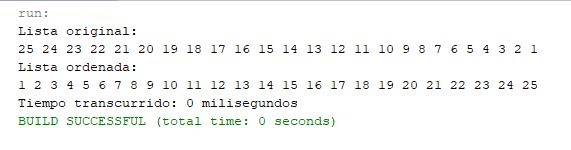
\includegraphics[width=0.8\textwidth,keepaspectratio]{img/ej1.jpg}
		%\includesvg{img/automata.svg}
		%\label{img:mot2}
		%\caption{Product backlog.}
	\end{figure}	
	
	\begin{itemize}
		\item Tamaño: 10000
	\end{itemize}
	
	\begin{figure}[H]
		\centering
		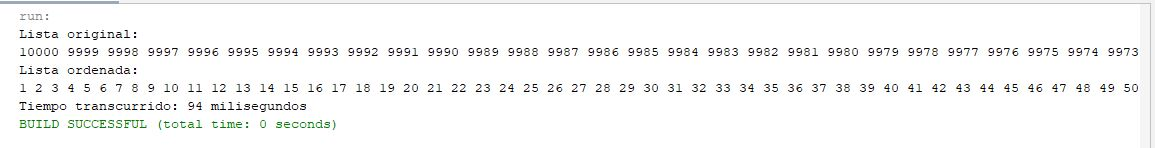
\includegraphics[width=0.8\textwidth,keepaspectratio]{img/ej2.jpg}
		%\includesvg{img/automata.svg}
		%\label{img:mot2}
		%\caption{Product backlog.}
	\end{figure}
	
	\subsubsection{Ejercicio 2}
	\begin{itemize}
		\item Utilizar el tipo generico de Doble Lista Enlazada para generar los peores casos y ejecutar el	algoritmo de ordenamiento.
	\end{itemize}
	
	\lstinputlisting[language=java, caption={Node.java},numbers=left,]{src/Ejercicio02/Node.java}
	
	\begin{itemize}
		\item La clase Node tiene un parámetro de tipo genérico E que representa el tipo de dato que se almacenará en el nodo.
		\item Hay varios constructores disponibles para crear un objeto Node. Estos constructores permiten especificar el dato del nodo, así como las referencias al siguiente nodo y al nodo anterior.
		\item En resumen, la clase Node proporciona la estructura básica de un nodo en una estructura de datos enlazada, con métodos para acceder y modificar los datos y referencias del nodo.
	\end{itemize}
	
	\lstinputlisting[language=java, caption={DobleList.java},numbers=left,]{src/Ejercicio02/DobleList.java}
		
	\begin{itemize}
		\item La clase DobleList tiene un parámetro de tipo genérico E que representa el tipo de dato que se almacenará en la lista.
		\item La lista doblemente enlazada contiene referencias a dos nodos, head (cabeza) que apunta al primer nodo de la lista y tail (cola) que apunta al último nodo de la lista. Además, se mantiene un contador size para realizar un seguimiento del tamaño de la lista.
		\item El constructor de la clase inicializa la lista vacía estableciendo la cabeza (head) como null.
		\item El método isEmpty verifica si la lista está vacía verificando si tanto la cabeza (head) como la cola (tail) son null.
		\item Los métodos insertAlInicio e insertFinal permiten insertar un nuevo nodo al inicio y al final de la lista, respectivamente.
		\item El método size devuelve el tamaño actual de la lista.
		\item El método generarPeoresCasos implementa un algoritmo de ordenación de selección para ordenar la lista en orden descendente.
		\item El método insertionSort implementa un algoritmo de ordenación por inserción para ordenar la lista en orden ascendente.
		\item El método swapNodes intercambia los elementos de dos nodos dados.
		\item El método toString crea una representación de cadena de la lista concatenando los elementos de los nodos.
	\end{itemize}
	
	\lstinputlisting[language=java, caption={Lab4.java},numbers=left,]{src/Ejercicio02/Lab4.java}
	
	\begin{itemize}
		\item El programa solicita al usuario que ingrese el tamaño de un arreglo mediante la clase Scanner.
		\item Se crea un arreglo de tipo DobleList<Integer> llamado array, que contendrá tamano listas doblemente enlazadas.
		\item Se itera sobre el arreglo array y se crea una nueva lista doblemente enlazada en cada posición. Luego se insertan elementos en cada lista de acuerdo a su posición en el arreglo.	
		\item Se genera peores casos para cada lista del arreglo utilizando el método generarPeoresCasos de la clase DobleList.
		\item Se llama al método times para calcular los tiempos de ejecución y escribirlos en un archivo.
		\item Se crea una instancia de la clase JavaPlot para mostrar un gráfico.
		\item Se agrega un gráfico desde un archivo de datos utilizando el método addPlot de la clase JavaPlot.	
		\item Se muestra el gráfico utilizando el método plot de la clase JavaPlot.
		\item Ejecucion:
	\end{itemize}
	
	\begin{figure}[H]
		\centering
		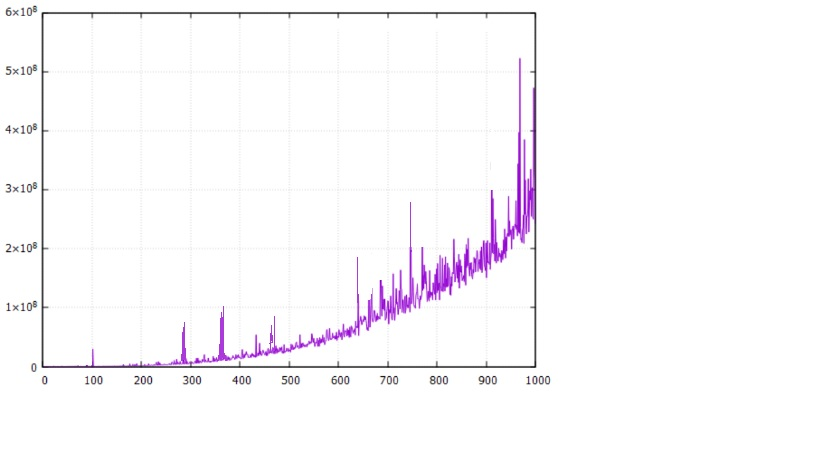
\includegraphics[width=0.8\textwidth,keepaspectratio]{img/ej3.jpg}
		%\includesvg{img/automata.svg}
		%\label{img:mot2}
		%\caption{Product backlog.}
	\end{figure}
	
	\section{Preguntas}
	\subsection{¿Como se ejecutaría sus implementaciones desde terminal(consola)?}
	\begin{itemize}
	\item Descarga la biblioteca JavaPlot desde el siguiente enlace https://sourceforge.net/projects/gnujavaplot/
	\item Extrae el archivo ZIP descargado y encuentra el archivo JAR de la biblioteca JavaPlot 
	\item Abre la consola y navega hasta el directorio donde se encuentra el archivo JAR de JavaPlot.
	\item Compila tu archivo Java que utiliza JavaPlot utilizando el siguiente comando:
	\begin{lstlisting}[language=bash,caption={}][H]
		javac -cp gnuplot-java.jar TuArchivoJava.java
	\end{lstlisting}
	
	\item Ejecuta tu archivo Java utilizando el siguiente comando:
	\begin{lstlisting}[language=bash,caption={}][H]
		java -cp .:gnuplot-java.jar TuArchivoJava
	\end{lstlisting}
	
	\end{itemize}	

	
	\section{Conclusiones}
	\begin{itemize}
		\item La implementación de una cola de prioridad utilizando un heap proporciona un tiempo de ejecución eficiente para las operaciones de inserción y eliminación de elementos con mayor prioridad.
		\item El uso de estructuras de datos genéricas y programación orientada a objetos permite crear implementaciones flexibles y reutilizables.
		\item El diseño de clases y métodos bien encapsulados promueve un código limpio y mantenible.
		\item La comprensión de las propiedades y operaciones del heap es fundamental para implementar correctamente una cola de prioridad.
		\item En este ejercicio, se ha implementado una cola de prioridad utilizando un heap como estructura de datos subyacente. La implementación del heap permite realizar las operaciones de inserción, eliminación y acceso a los elementos con mayor y menor prioridad de manera eficiente. El uso de una clase genérica y la implementación de la interfaz Comparable proporcionan flexibilidad para trabajar con diferentes tipos de elementos y prioridades.
		\item La implementación de una cola de prioridad basada en un heap es una estrategia poderosa y eficiente para resolver problemas que implican la gestión de elementos con diferentes niveles de prioridad. Al comprender los conceptos y técnicas presentadas en este ejercicio, se puede aplicar este conocimiento a una amplia gama de problemas en los que se requiere un manejo eficiente de la prioridad.
		\item Informe a detalle en: 
		\item \url {https://docs.google.com/document/d/1jAOoSbbO_PYWXzPXPUOXgS0euRT48e6vSWjYnETln9Y/edit?usp=sharing}

	\end{itemize}
	\section{Referencias}
	\begin{itemize}
		\item \url{https://aulavirtual.unsa.edu.pe/2023A/mod/page/view.php?id=44926}			
		\item \url{https://drive.google.com/file/d/1Ma9WERoSytydCbQc9S3XOsiUbim1XXQq/view}
	\end{itemize}	
	
\end{document}